\documentclass[aspectratio=169]{beamer}

\usetheme{Madrid}
\usecolortheme{default}
\setbeamertemplate{navigation symbols}{}

\usepackage[utf8]{inputenc}
\usepackage[T1]{fontenc}
\usepackage{amsmath, amssymb, amsfonts}
\usepackage{booktabs}
\usepackage{array}
\usepackage{ragged2e}
\usepackage{hyperref}
\usepackage{graphicx}

\title{Verification of Quantum Circuits and Optimization}
\subtitle{A Layered Survey of Semantic, Symbolic, Compiler, and Program-Logical Approaches}
\author{Asha}
\institute{}
\date{}

\begin{document}

% ------------------------------------------------
\begin{frame}
  \titlepage
\end{frame}

% ------------------------------------------------
\begin{frame}{Thesis}
\justifying
\begin{block}{Main Claim}
Quantum circuit verification is not one monolithic problem. It is a layered stack involving:
\begin{enumerate}
    \item semantic foundations,
    \item scalable proof techniques,
    \item compiler-oriented verification,
    \item and program-logical reasoning.
\end{enumerate}
\end{block}

\pause

\begin{alertblock}{Central Perspective}
Optimization is not peripheral to this story. It is the practical pressure that shapes the design of verification methods.
\end{alertblock}
\end{frame}

% ------------------------------------------------
\begin{frame}{Why Verification is Hard in Quantum Computing}
\justifying
\begin{itemize}
    \item Quantum programs are expensive to simulate.
    \item Outputs are often probabilistic, so testing is weaker than in classical software.
    \item Debugging is difficult because observing a quantum state can disturb it.
    \item Hardware imposes physical constraints: limited qubits, connectivity, decoherence, noise.
    \item Therefore optimization is essential.
    \item But optimization is also dangerous: an incorrect rewrite may silently change semantics.
\end{itemize}

\vspace{0.5em}
\begin{block}{Tension}
Quantum software needs aggressive transformation, but those transformations are exactly where correctness becomes hardest to trust.
\end{block}
\end{frame}

% ------------------------------------------------
\begin{frame}{What is the Verification Problem?}
\justifying
We want machine-checked evidence that a quantum artifact preserves its intended meaning.

\vspace{0.7em}

\begin{itemize}
    \item \textbf{Artifacts:} circuits, circuit-generating programs, compiler passes
    \item \textbf{Properties:} equivalence, equivalence up to phase, ancilla validity, translation correctness
    \item \textbf{Main obstacle:} direct matrix reasoning scales exponentially with qubit count
\end{itemize}

\vspace{0.7em}
\begin{block}{Why this matters}
Different papers attack different parts of this problem.
\end{block}
\end{frame}

% ------------------------------------------------
\begin{frame}{A Layered View of the Literature}
\begin{block}{Layer I: Semantic foundations}
QWIRE, QWIRE Practice, ReQWIRE
\end{block}

\begin{block}{Layer II: Scalable proof methods}
Symbolic Reasoning, sQIRe, VOQC
\end{block}

\begin{block}{Layer III: Compiler automation}
CertiQ, OpenQASM $\to$ sqir translation
\end{block}

\begin{block}{Layer IV: Program logic}
Qbricks, CoqQ
\end{block}
\end{frame}

% ------------------------------------------------
\begin{frame}{Layer I: Semantic and Type-Theoretic Foundations}
\justifying
\textbf{Core question:} What does a quantum circuit mean, and what counts as well-formed?

\vspace{0.5em}
\begin{itemize}
    \item \textbf{QWIRE}: linear type discipline + denotational semantics for quantum circuits.
    \item \textbf{QWIRE Practice}: mechanization in Coq using superoperators on density matrices.
    \item \textbf{ReQWIRE}: refines the semantic story around ancilla assertions and reversible reasoning.
\end{itemize}

\pause

\begin{block}{Main contribution of this layer}
It gives a mathematically stable notion of meaning and rules out malformed circuit manipulations.
\end{block}

\pause

\begin{alertblock}{Tradeoff}
Strong semantic trust, but proofs can become expensive and hard to scale.
\end{alertblock}
\end{frame}
% ------------------------------------------------
\begin{frame}{QWIRE: What Kind of Language Is It?}
\justifying
\textbf{QWIRE} is a small \emph{quantum circuit language} embedded inside a classical host language.

\vspace{0.7em}
\begin{itemize}
    \item The host language handles classical control and metaprogramming.
    \item QWIRE handles the quantum circuit fragment itself.
    \item Its \textbf{linear type system} tracks quantum wires so they are used exactly in physically meaningful ways.
    \item Its semantics gives circuits a precise mathematical meaning.
\end{itemize}

\vspace{0.7em}
\begin{block}{Why this design?}
Quantum circuits are low-level objects, but programmers want to build and manipulate them using ordinary classical programming structure.
\end{block}
\end{frame}
% ------------------------------------------------
\begin{frame}{A Tiny QWIRE-Style Example}
\justifying
A very small circuit can be described as:

\vspace{0.5em}
\[
\text{input qubit } q \;\mapsto\; H(q);\; \text{measure}(q)
\]

\vspace{0.7em}
In QWIRE-style pseudocode, the idea is:

\begin{center}
\begin{minipage}{0.82\textwidth}
\ttfamily
box\_ (\_ : Qubit) =>\\
\hspace*{1.5em}q $\leftarrow$ init0;\\
\hspace*{1.5em}q $\leftarrow$ gate\_ H q;\\
\hspace*{1.5em}x $\leftarrow$ measure q;\\
\hspace*{1.5em}output x
\end{minipage}
\end{center}

% \vspace{0.7em}
\begin{itemize}
    \item \texttt{init0} allocates a fresh qubit in $\lvert 0 \rangle$
    \item \texttt{H} creates the superposition
    \[
      H\lvert 0 \rangle = \frac{1}{\sqrt{2}}(\lvert 0 \rangle + \lvert 1 \rangle)
    \]
    \item \texttt{measure} returns a classical bit
\end{itemize}
\end{frame}
% ------------------------------------------------
\begin{frame}{What Does QWIRE Verify Here?}
\justifying
For a simple circuit like the previous one, the proof story has two parts.

\vspace{0.7em}
\textbf{1. Well-formedness by typing}
\begin{itemize}
    \item each wire is used linearly,
    \item no qubit is duplicated,
    \item no discarded wire is used again.
\end{itemize}

\vspace{0.5em}
\textbf{2. Behavioral correctness by semantics}
\begin{itemize}
    \item the circuit is interpreted as a superoperator on density matrices,
    \item then one proves that the denotation matches the intended behavior.
\end{itemize}

\vspace{0.7em}
For this example, the desired statement is:
\begin{block}{Expected property}
Measuring \(H\lvert 0 \rangle\) returns \(0\) and \(1\) with equal probability \(1/2\).
\end{block}
\end{frame}
% ------------------------------------------------
\begin{frame}{QWIRE Practice: How the Proof Process Looks in Coq}
\justifying
QWIRE Practice turns the language into a mechanized verification framework in Coq.

\vspace{0.7em}
\begin{enumerate}
    \item Write the circuit in the embedded syntax.
    \item Use the type-checking infrastructure to show the circuit is well-typed.
    \item Interpret the circuit denotationally as a superoperator.
    \item State the intended property.
    \item Prove, in Coq, that the denotation satisfies that property.
\end{enumerate}

\vspace{0.7em}
\begin{alertblock}{Main point}
The proof is not just about one simulation run.  
It is about the mathematical meaning of the circuit for all executions.
\end{alertblock}
\end{frame}
% ------------------------------------------------
\begin{frame}{Layer I Example: Why ReQWIRE Matters}
\justifying
Ancillae are temporary qubits introduced during computation.

\vspace{0.5em}
\begin{itemize}
    \item In practice, programmers often \emph{assert} that an ancilla has been returned to $\lvert 0 \rangle$ before discard.
    \item That assertion is optimization-relevant but semantically nontrivial.
    \item ReQWIRE distinguishes:
    \begin{itemize}
        \item a trusted safe semantics,
        \item and an assertion-based semantics.
    \end{itemize}
    \item Validity means these coincide when the assertion is actually justified.
\end{itemize}

\pause

\begin{block}{Takeaway}
This is a good example of a semantic design that captures a compiler-relevant correctness condition.
\end{block}
\end{frame}

% ------------------------------------------------
\begin{frame}{Layer II: Scalable Symbolic Reasoning and Proof-Friendly IRs}
\justifying
\textbf{Core question:} Once semantics exists, how do we make proofs scale?

\vspace{0.5em}
\begin{itemize}
    \item \textbf{Symbolic Reasoning in Coq}: replace brute-force matrix expansion with symbolic Dirac-style rewriting.
    \item \textbf{sQIRe}: redesign the intermediate representation using indexed global registers.
    \item \textbf{VOQC}: build a verified optimizer on top of a proof-friendly low-level IR.
\end{itemize}

\pause

\begin{block}{Key insight}
Scalability is not only a theorem-proving problem. It is also a \textbf{representation problem}.
\end{block}
\end{frame}

% ------------------------------------------------
\begin{frame}{Why Move Beyond QWIRE?}
\justifying
QWIRE gives a strong semantic foundation, but optimization proofs need a representation
that is easier to rewrite and manipulate mechanically.

\vspace{0.7em}
\begin{itemize}
    \item QWIRE is excellent for expressing well-typed circuits and reasoning about meaning.
    \item But large-scale optimizer proofs require many local rewrites and structural transformations.
    \item That creates pressure for a lower-level intermediate representation.
\end{itemize}

\vspace{0.7em}
\begin{alertblock}{Main shift}
The question changes from
\[
\textit{``What does a circuit mean?''}
\]
to
\[
\textit{``What representation makes verified transformations practical?''}
\]
\end{alertblock}
\end{frame}
% ------------------------------------------------
\begin{frame}{sQIRe / SQIR: A Proof-Friendly Quantum IR}
\justifying
\textbf{sQIRe} introduces a simpler, lower-level representation for quantum circuits.

\vspace{0.7em}
\begin{itemize}
    \item It uses a \textbf{global indexed register} of qubits.
    \item Gates act on qubit positions such as \(0,1,2,\dots\), rather than on abstract wire variables.
    \item This makes composition and rewriting much more direct.
    \item The same design also fits well with compilation to and from existing circuit toolchains.
\end{itemize}

\vspace{0.7em}
\begin{block}{Key idea}
sQIRe sacrifices some high-level elegance in order to make low-level reasoning and verified optimization easier.
\end{block}
\end{frame}
% ------------------------------------------------
\begin{frame}{Example: Bell-State Circuit in a Lower-Level IR}
\justifying
A Bell-state circuit can be described operationally as:

\[
\ket{00}
\;\xrightarrow{H\text{ on }0}\;
\frac{1}{\sqrt{2}}(\ket{00}+\ket{10})
\;\xrightarrow{\mathrm{CNOT}(0,1)}\;
\frac{1}{\sqrt{2}}(\ket{00}+\ket{11})
\]

\vspace{0.8em}
In a QWIRE-style view, we think in terms of typed wires and circuit structure.

\vspace{0.4em}
In an sQIRe/SQIR-style view, we think more like:
\begin{center}
\ttfamily
H 0; \quad CNOT 0 1
\end{center}

\vspace{0.8em}
\begin{block}{Why this matters}
For optimization, the lower-level indexed form is often easier to scan, rewrite, commute, cancel, and verify.
\end{block}
\end{frame}
% ------------------------------------------------
\begin{frame}{Example: Bell-State Circuit in a Lower-Level IR}
\justifying
A Bell-state circuit can be described operationally as:

\[
\ket{00}
\;\xrightarrow{H\text{ on }0}\;
\frac{1}{\sqrt{2}}(\ket{00}+\ket{10})
\;\xrightarrow{\mathrm{CNOT}(0,1)}\;
\frac{1}{\sqrt{2}}(\ket{00}+\ket{11})
\]

\vspace{0.8em}
In a QWIRE-style view, we think in terms of typed wires and circuit structure.

\vspace{0.4em}
In an sQIRe/SQIR-style view, we think more like:
\begin{center}
\ttfamily
H 0; \quad CNOT 0 1
\end{center}

\vspace{0.8em}
\begin{block}{Why this matters}
For optimization, the lower-level indexed form is often easier to scan, rewrite, commute, cancel, and verify.
\end{block}
\end{frame}
% ------------------------------------------------
\begin{frame}{What sQIRe Makes Easier to Verify}
\justifying
The motivation for sQIRe was not only semantic clarity, but \textbf{transformation proof engineering}.

\vspace{0.7em}
Examples highlighted in this line of work include:
\begin{itemize}
    \item \textbf{skip elimination}
    \item \textbf{NOT propagation}
    \item \textbf{mapping / layout transformations}
    \item local circuit rewrites used in optimizers
\end{itemize}

\vspace{0.7em}
\begin{alertblock}{Key lesson}
Some transformations were much harder to verify in QWIRE-style representations, but became more manageable in sQIRe's lower-level global-register form.
\end{alertblock}
\end{frame}
% ------------------------------------------------
\begin{frame}{VOQC: From IR Design to a Verified Optimizer}
\justifying
Once a proof-friendly IR is in place, the next step is to verify real optimizations.

\vspace{0.7em}
\begin{itemize}
    \item \textbf{VOQC} is built on top of SQIR.
    \item Optimizations are written as Coq functions over circuits in this IR.
    \item Each transformation is proved correct with respect to the semantics of SQIR programs.
    \item The result is a fully verified optimizer for quantum circuits.
\end{itemize}

\vspace{0.7em}
\begin{block}{Interpretation}
sQIRe/SQIR changes the representation.  
VOQC turns that representation into a practical verified optimization pipeline.
\end{block}
\end{frame}
% ------------------------------------------------
\begin{frame}{QWIRE vs. sQIRe / SQIR}
\centering
\renewcommand{\arraystretch}{1.35}
\begin{tabular}{>{\raggedright\arraybackslash}p{3.2cm} >{\raggedright\arraybackslash}p{3.8cm} >{\raggedright\arraybackslash}p{3.8cm}}
\toprule
 & \textbf{QWIRE} & \textbf{sQIRe / SQIR} \\
\midrule
Main goal & semantic foundations & proof-friendly optimization IR \\
Style & typed circuit language & simple low-level circuit language \\
Representation & abstract wires / structured circuits & indexed global qubit register \\
Strength & elegance, semantics, typing & easier rewriting and optimizer proofs \\
Best suited for & foundational verification & verified transformations and optimization \\
\bottomrule
\end{tabular}
\end{frame}
% ------------------------------------------------
\begin{frame}{VOQC Architecture}
\centering
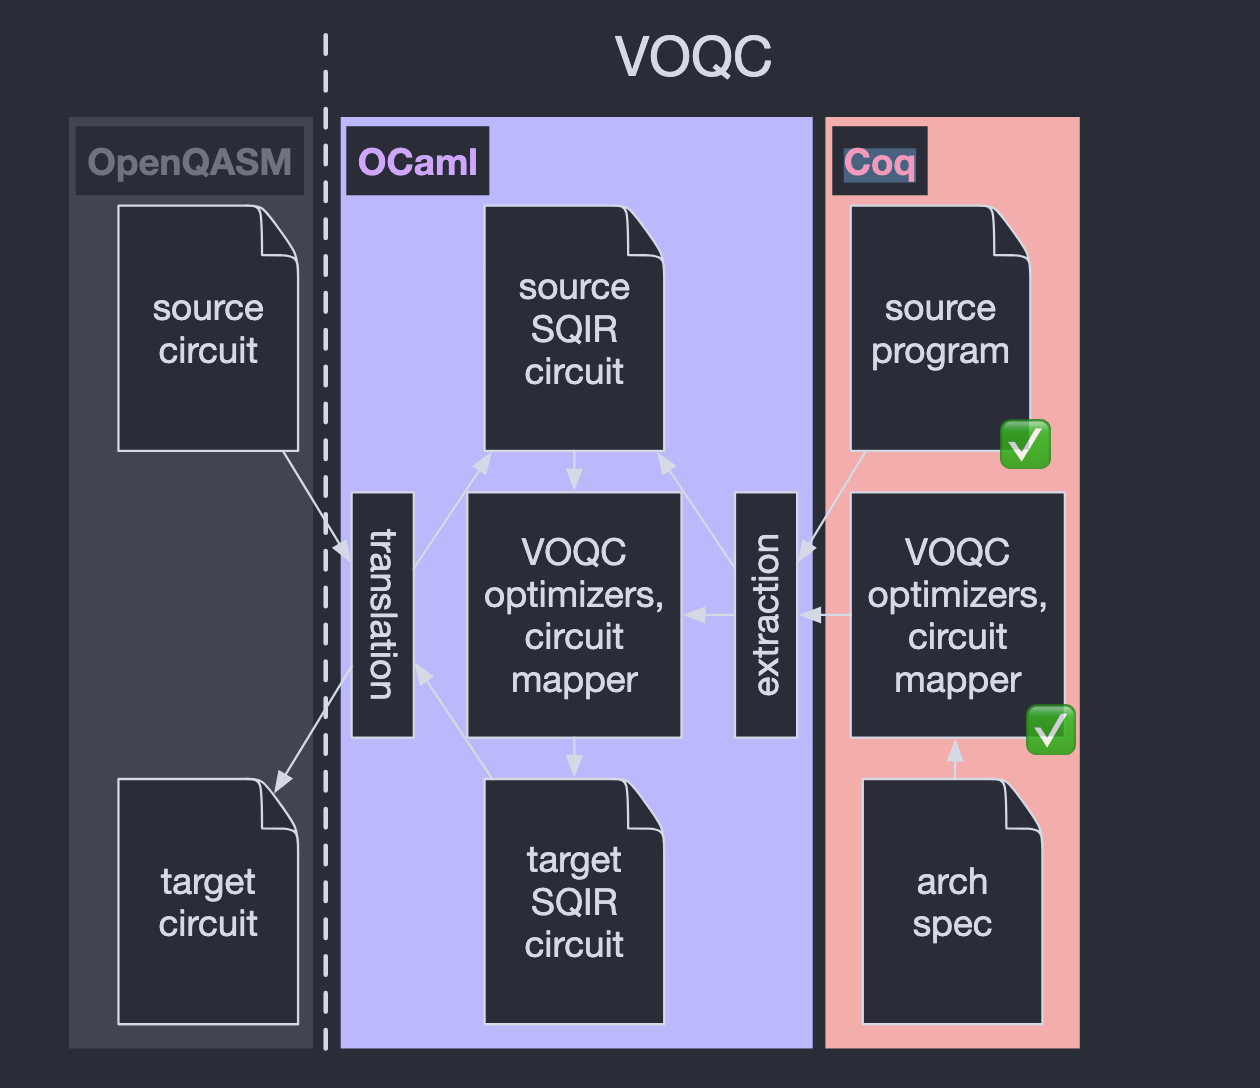
\includegraphics[width=0.3\textwidth]{fig1.png}

\vspace{0.6em}
\begin{block}{Idea}
VOQC builds a verified optimizer on top of the SQIR intermediate representation:
circuits are represented in a proof-friendly IR, transformed by optimizer passes,
and each pass is proved semantics-preserving in Coq.
\end{block}
\end{frame}
% ------------------------------------------------
\begin{frame}{What Does VOQC Actually Optimize?}
\justifying
VOQC is not just one rewrite. It is a library of verified circuit transformations.

\vspace{0.7em}
Typical goals include:
\begin{itemize}
    \item removing redundant gates,
    \item simplifying local gate patterns,
    \item propagating gates through circuits when commutation allows it,
    \item reducing gate count before later compilation stages.
\end{itemize}

\vspace{0.7em}
\begin{alertblock}{Key point}
Each optimization is implemented as a Coq function over SQIR circuits and proved to preserve semantics.
\end{alertblock}
\end{frame}
% ------------------------------------------------
\begin{frame}{Example Optimization: Gate Cancellation}
\centering
\Large
\[
H(q);\, H(q) \;\Longrightarrow\; \texttt{skip}
\]

\vspace{0.6em}

\[
X(q);\, X(q) \;\Longrightarrow\; \texttt{skip}
\]

\vspace{0.6em}

\[
\mathrm{CNOT}(a,b);\, \mathrm{CNOT}(a,b) \;\Longrightarrow\; \texttt{skip}
\]

\vspace{0.6em}
\normalsize
\begin{block}{Why is this valid?}
These gates are self-inverse, so applying them twice gives the identity transformation.
\end{block}
\end{frame}
% ------------------------------------------------
\begin{frame}{Example Optimization: Propagate, Then Cancel}
\justifying
Sometimes a gate cannot be canceled immediately, but it can be moved until cancellation becomes possible.

\vspace{0.8em}
Example pattern:
\[
X(q);\, \text{something commuting with }X(q);\, X(q)
\]

If the middle part does not affect the same qubit in a conflicting way, VOQC-style rewrites may transform:
\[
X(q);\, C;\, X(q)
\quad\Longrightarrow\quad
C;\, X(q);\, X(q)
\quad\Longrightarrow\quad
C
\]

\vspace{0.8em}
\begin{block}{Interpretation}
The optimizer first \textbf{propagates} a gate through the circuit, then uses a local
\textbf{cancellation} rule to remove redundancy.
\end{block}
\end{frame}
% ------------------------------------------------
\begin{frame}{Propagation-Based Rewriting Intuition}
\justifying
The hard part is not cancellation itself.  
The hard part is showing that a gate may be moved across other gates without changing meaning.

\vspace{0.8em}
Typical reasoning pattern:
\begin{itemize}
    \item identify a local commutation or propagation law,
    \item rewrite the circuit into a more convenient form,
    \item expose a redundant pair,
    \item cancel the pair.
\end{itemize}

\vspace{0.8em}
\begin{alertblock}{Why SQIR helps}
Because circuits are represented over indexed qubits in a simple IR, these structural rewrites are easier to express and verify than in richer higher-level representations.
\end{alertblock}
\end{frame}
% ------------------------------------------------
\begin{frame}{Another VOQC Strategy: \texttt{gridify}}
\justifying
VOQC does not rely only on good IR design and rewrite rules.  
It also introduces a proof-automation strategy for low-level equivalence proofs.

\vspace{0.7em}
\begin{itemize}
    \item Section 4.5 introduces the Coq tactic \texttt{gridify}.
    \item Its job is to prove local circuit equalities used inside optimizer passes.
    \item It rewrites matrix expressions into a common \textbf{grid normal form}.
    \item Then it applies matrix identities to show the two circuits have the same semantics.
\end{itemize}

\vspace{0.7em}
\begin{block}{Why this matters}
VOQC is not only about \emph{what} optimizations to perform.  
It is also about \emph{how to verify} those optimizations without doing every matrix proof by hand.
\end{block}
\end{frame}
% ------------------------------------------------
\begin{frame}{What \texttt{gridify} Actually Does}
\justifying
For valid cases, \texttt{gridify} rewrites matrix expressions into a
\textbf{grid normal form}:

\[
((\cdots \times \cdots)\otimes(\cdots \times \cdots))
+
((\cdots \times \cdots)\otimes(\cdots \times \cdots))
\]

\vspace{0.7em}
It uses standard matrix identities such as:
\[
I_{mn} = I_m \otimes I_n
\qquad
A(B+C)=AB+AC
\qquad
(A+B)C=AC+BC
\]
\[
A \otimes (B+C)=A\otimes B + A\otimes C
\qquad
(A\otimes B)(C\otimes D)=(AC)\otimes(BD)
\]

\vspace{0.7em}
\begin{alertblock}{Why this matters}
VOQC is not only about designing optimizations.
It is also about building proof automation strong enough to verify them at scale.
\end{alertblock}
\end{frame}
% ------------------------------------------------

\begin{frame}{Another VOQC Strategy: Automating Local Rewrite Proofs}
\justifying
A verified optimizer needs many small semantic equivalence proofs.

\vspace{0.7em}
In VOQC, Section 4.5 introduces \texttt{gridify} as a tactic for proving these
low-level equalities automatically.

\vspace{0.7em}
Typical workflow:
\begin{enumerate}
    \item expand the two circuits into matrix expressions,
    \item normalize them into a common grid-like form,
    \item use algebraic identities to conclude equality.
\end{enumerate}

\vspace{0.7em}
\begin{alertblock}{Narrative role}
So beyond SQIR and rewrite passes, VOQC also contributes \textbf{proof automation}
as a strategy for scalable verified optimization.
\end{alertblock}
\end{frame}
% ------------------------------------------------

\begin{frame}{How a VOQC Proof Works}
\justifying
For one optimization pass, the proof pattern is roughly:

\vspace{0.6em}
\begin{enumerate}
    \item define the transformation as a function on SQIR circuits,
    \item state the semantic meaning of the original circuit,
    \item state the semantic meaning of the transformed circuit,
    \item prove that the two denotations are equal.
\end{enumerate}

\vspace{0.8em}
\begin{block}{What is being proved?}
Not that the optimizer works on one example, but that \emph{every circuit transformed by the pass}
has the same semantics before and after optimization.
\end{block}
\end{frame}
% ------------------------------------------------

% ------------------------------------------------
% ------------------------------------------------
% ------------------------------------------------
% ------------------------------------------------
% ------------------------------------------------

\begin{frame}{Local Rewrite, Global Guarantee}
\centering
\Large
\[
\text{rewrite rule} \quad + \quad \text{semantic proof}
\quad \Longrightarrow \quad
\text{verified optimization pass}
\]

\vspace{1em}
\normalsize
\begin{itemize}
    \item The rewrite is local.
    \item The proof is semantic.
    \item The final guarantee is global: optimized circuits mean the same thing as original circuits.
\end{itemize}
\end{frame}

% ------------------------------------------------

\begin{frame}{Why IR Design Matters: sQIRe and VOQC}
\justifying
\begin{columns}[T]
\column{0.49\textwidth}
\textbf{sQIRe}
\begin{itemize}
    \item simpler low-level indexed representation,
    \item easier rewriting and composition,
    \item better suited for optimization proofs.
\end{itemize}

\column{0.49\textwidth}
\textbf{VOQC}
\begin{itemize}
    \item first fully verified optimizer for general quantum circuits,
    \item verifies correctness-preserving rewrites,
    \item shows that proof-oriented IR design can support serious optimization pipelines.
\end{itemize}
\end{columns}

\vspace{1em}
\begin{alertblock}{Big lesson}
A convenient source language is not always the right representation for verified optimization.
\end{alertblock}
\end{frame}

% ------------------------------------------------
\begin{frame}{Layer III: Compiler-Oriented Automation}
\justifying
\textbf{Core question:} How do we verify realistic compiler workflows with less interactive proof effort?

\vspace{0.5em}
\begin{itemize}
    \item \textbf{CertiQ}: symbolic execution + SMT-based equivalence checking for realistic compiler passes.
    \item \textbf{Verified OpenQASM-to-sqir translation}: proves correctness of a bridge from a practical external language into a proof-oriented IR.
\end{itemize}

\pause

\begin{block}{What changes in this layer?}
The emphasis shifts from human-guided semantic proof to automation and toolchain realism.
\end{block}
\end{frame}

% ------------------------------------------------
\begin{frame}{VOQC vs. CertiQ}
\centering
\renewcommand{\arraystretch}{1.35}
\begin{tabular}{>{\raggedright\arraybackslash}p{3.2cm} >{\raggedright\arraybackslash}p{3.8cm} >{\raggedright\arraybackslash}p{3.8cm}}
\toprule
 & \textbf{VOQC} & \textbf{CertiQ} \\
\midrule
Primary style & Interactive proof assistant verification & Mostly automated solver-aided checking \\
Focus & Verified rewrites and optimizer pipeline & Realistic compiler passes and engineering workflow \\
Strength & Strong semantic assurance & Greater automation and industrial flavor \\
Tradeoff & More proof effort & Narrower obligation style / solver-oriented \\
\bottomrule
\end{tabular}

\vspace{1em}
\begin{block}{Interpretation}
These approaches are complementary, not competitors.
\end{block}
\end{frame}

% ------------------------------------------------
\begin{frame}{CertiQ Architecture}
\centering
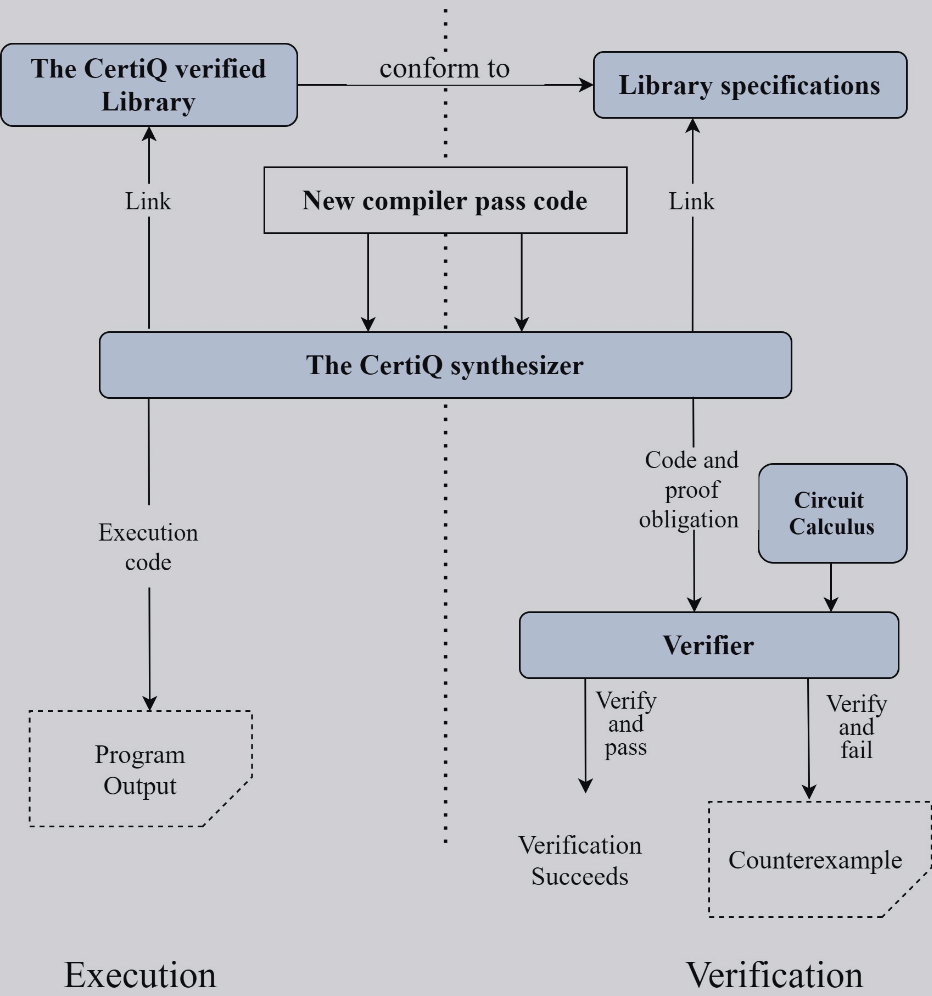
\includegraphics[width=0.3\textwidth]{fig2.png}


\end{frame}
% ------------------------------------------------
\begin{frame}{Why CertiQ?}
\justifying
VOQC shows that verified optimization is possible in a proof assistant.

\vspace{0.7em}
CertiQ asks a different question:

\begin{block}{Main question}
Can we verify \textbf{realistic compiler passes} from a widely used compiler
without requiring heavy interactive proof for each pass?
\end{block}

\vspace{0.7em}
Its answer is to target \textbf{Qiskit} and use a mostly automated verification workflow
based on symbolic reasoning and SMT solving.
\end{frame}
% ------------------------------------------------
\begin{frame}{What CertiQ Provides}
\justifying
CertiQ is a verification framework for writing and verifying compiler passes for Qiskit.

\vspace{0.7em}
Its main ingredients are:
\begin{itemize}
    \item a \textbf{CertiQ interface} for compiler passes,
    \item generation of \textbf{verification conditions},
    \item a \textbf{quantum circuit calculus} for circuit reasoning,
    \item \textbf{SMT-based checking} of circuit equivalence,
    \item and verified libraries for common data structures and circuit transformations.
\end{itemize}

\vspace{0.7em}
\begin{alertblock}{Narrative role}
CertiQ shifts the focus from hand-crafted proof scripts to a more automated compiler-verification workflow.
\end{alertblock}
\end{frame}
% ------------------------------------------------
\begin{frame}{CertiQ vs. VOQC}
\centering
\renewcommand{\arraystretch}{1.35}
\begin{tabular}{>{\raggedright\arraybackslash}p{3.2cm} >{\raggedright\arraybackslash}p{3.7cm} >{\raggedright\arraybackslash}p{3.7cm}}
\toprule
 & \textbf{VOQC} & \textbf{CertiQ} \\
\midrule
Main style & Coq-based verified optimizer & Mostly automated compiler-pass verification \\
Target & SQIR-based optimization pipeline & Realistic Qiskit transpiler passes \\
Core technique & semantic proofs in Coq & symbolic execution + SMT checking \\
Strength & strong proof-assistant assurance & better automation and closer compiler realism \\
\bottomrule
\end{tabular}

\vspace{0.8em}
\begin{block}{Takeaway}
VOQC and CertiQ are complementary:
one emphasizes proof-assistant trust, the other emphasizes automation for real compiler engineering.
\end{block}
\end{frame}
% ------------------------------------------------
\begin{frame}{How CertiQ Verification Works}
\justifying
At a high level, CertiQ verifies a compiler pass by:

\vspace{0.6em}
\begin{enumerate}
    \item expressing the pass in the CertiQ framework,
    \item generating verification conditions,
    \item translating circuit-equivalence obligations into the quantum circuit calculus,
    \item encoding these obligations into SMT,
    \item and checking that the transformed circuit preserves semantics.
\end{enumerate}

\vspace{0.8em}
\begin{block}{Main idea}
The goal is not to prove every pass manually in Coq,
but to automate as much of the compiler-verification burden as possible.
\end{block}
\end{frame}
% ------------------------------------------------
\begin{frame}{Verified Translation Between Low-Level Quantum Languages}
\justifying
This paper studies a verified translator from \textbf{OpenQASM} to \textbf{sqir/SQIR}.  
Its goal is to connect a practical low-level quantum language to the proof-oriented IR used by VOQC. 

\vspace{0.7em}
\begin{block}{Main question}
How can we safely bring circuits written in OpenQASM into the verified SQIR world?
\end{block}
\end{frame}
% ------------------------------------------------
\begin{frame}{What the Paper Proves}
\justifying
The paper develops:
\begin{itemize}
    \item a formal semantics for OpenQASM,
    \item a translation into \textbf{sqir/SQIR},
    \item and a proof that translation preserves meaning.
\end{itemize}

\vspace{0.7em}
\begin{block}{Core guarantee}
An OpenQASM circuit and its translated SQIR circuit have the same semantics.
\end{block}
\end{frame}
% ------------------------------------------------
\begin{frame}{Relationship to VOQC}
\justifying
This paper and VOQC solve two different parts of the same pipeline.

\vspace{0.7em}
\[
\text{OpenQASM}
\;\xrightarrow{\text{verified translation}}\;
\text{SQIR}
\;\xrightarrow{\text{VOQC}}\;
\text{verified optimization}
\]

\vspace{0.7em}
\begin{itemize}
    \item The translation paper gets external circuits into SQIR safely.
    \item VOQC then optimizes those SQIR circuits with verified rewrites.
\end{itemize}

\vspace{0.7em}
\begin{alertblock}{Key point}
Without verified translation, VOQC would still rely on an unverified front end.
\end{alertblock}
\end{frame}
% ------------------------------------------------


\begin{frame}{Layer IV: From Circuits to Programs}
\justifying
\textbf{Core question:} What if the object being verified is not one circuit, but a circuit-building program or full quantum program?

\vspace{0.5em}
\begin{itemize}
    \item \textbf{Qbricks}: deductive verification framework for parameterized circuit-building programs.
    \item \textbf{CoqQ}: foundational program logic for quantum programs with rich specifications.
\end{itemize}

\pause

\begin{block}{What changes here?}
The unit of verification shifts:
\[
\text{fixed circuit} \quad \longrightarrow \quad \text{circuit family / full program}
\]
\end{block}

\pause

\begin{itemize}
    \item modular reasoning,
    \item pre/postconditions,
    \item source-level correctness,
    \item abstraction over algorithm families.
\end{itemize}
\end{frame}

% ------------------------------------------------
\begin{frame}{Why CoqQ?}
\justifying
Earlier verified frameworks focused mainly on circuits or low-level transformations.

\vspace{0.7em}
CoqQ shifts the focus to \textbf{full quantum programs} with:
\begin{itemize}
    \item classical control flow,
    \item high-level program structure,
    \item and rich source-level specifications.
\end{itemize}

\vspace{0.7em}
\begin{block}{Core challenge}
Quantum assertions are mathematically heavy, and entanglement makes ordinary
local reasoning difficult.
\end{block}

\vspace{0.5em}
\begin{alertblock}{CoqQ's response}
Build a \textbf{foundational verified program verifier} for a high-level quantum language,
with a sound program logic mechanized in Coq.
\end{alertblock}
\end{frame}
% ------------------------------------------------
\begin{frame}{What CoqQ Actually Provides}
\justifying
CoqQ is more than a library of examples. Its main components are:

\vspace{0.7em}
\begin{itemize}
    \item a \textbf{deeply embedded quantum programming language},
    \item a \textbf{denotational semantics},
    \item an expressive \textbf{Hoare-style program logic},
    \item and a \textbf{soundness proof} carried out in Coq.
\end{itemize}

\vspace{0.7em}
\begin{block}{Practical features}
Assertions can be written using \textbf{Dirac expressions}, and proofs can use
\textbf{local and parallel reasoning} to reduce proof effort.
\end{block}
\end{frame}
% ------------------------------------------------
\begin{frame}{Why Dirac-Style Assertions Matter}
\justifying
A key design choice in CoqQ is that specifications can use Dirac-style expressions.

\vspace{0.7em}
This matters because it lets correctness statements look closer to the way
quantum algorithms are usually explained on paper.

\vspace{0.7em}
For example, instead of an opaque matrix-level postcondition, one can state a goal
using explicit states such as:
\[
|a\rangle_x |\phi\rangle_y
\]
or superpositions built from basis states.

\vspace{0.7em}
\begin{alertblock}{Benefit}
Specifications become more readable, and proofs follow the mathematical structure
of textbook quantum algorithms more closely.
\end{alertblock}
\end{frame}
% ------------------------------------------------
\begin{frame}{Local and Parallel Reasoning in CoqQ}
\justifying
One of the hardest parts of quantum verification is that operations may be non-local
because of entanglement.

\vspace{0.7em}
CoqQ addresses this by supporting:
\begin{itemize}
    \item \textbf{local reasoning}: reason about the part of the state a command touches,
    \item \textbf{parallel reasoning}: combine reasoning about disjoint subsystems,
    \item and rules that help extend local facts into global correctness statements.
\end{itemize}

\vspace{0.7em}
\begin{block}{Why this is important}
Without this, proofs become cluttered by irrelevant parts of the global quantum state.
\end{block}
\end{frame}
% ------------------------------------------------
\begin{frame}{Example: CoqQ Verification of Grover}
\justifying
For Grover's algorithm, CoqQ proves a Hoare-style correctness statement relating
the program to its success probability.

\vspace{0.7em}
The paper shows that after \(r\) Grover iterations, the probability of obtaining
a solution is at least
\[
\sin^2((2r+1)t),
\qquad
t = \arcsin \sqrt{\frac{|f|}{|T|}}.
\]

\vspace{0.7em}
\begin{alertblock}{Interpretation}
CoqQ can verify algorithm-level probabilistic correctness claims, not only
syntactic circuit identities.
\end{alertblock}
\end{frame}
% ------------------------------------------------
\begin{frame}{Why Qbricks?}
\justifying
Earlier work focused mostly on fixed circuits or compiler transformations.

\vspace{0.7em}
Qbricks asks a different question:

\begin{block}{Main question}
How do we verify a \textbf{program that builds a family of quantum circuits},
rather than verifying one circuit at a time?
\end{block}

\vspace{0.7em}
This matters because many quantum algorithms are implemented as
\textbf{circuit-building programs}, not as one fixed circuit. 
\end{frame}
% ------------------------------------------------% ------------------------------------------------
\begin{frame}{What Qbricks Provides}
\justifying
Qbricks introduces a deductive verification framework centered on:
\begin{itemize}
    \item a DSL for \textbf{circuit families},
    \item a \textbf{specification language},
    \item \textbf{higher-order path sums (HOPS)},
    \item and a \textbf{hybrid quantum Hoare logic}.
\end{itemize}

\vspace{0.7em}
\begin{block}{Core idea}
Instead of proving properties of one concrete circuit,
Qbricks proves properties of a \textbf{parameterized circuit generator}.
\end{block}
\end{frame}
% ------------------------------------------------
\begin{frame}{What Makes Qbricks Different}
\justifying
Qbricks changes the unit of verification:

\vspace{0.7em}
\[
\text{single circuit}
\quad\longrightarrow\quad
\text{circuit-building program / circuit family}
\]

\vspace{0.7em}
So the goal is no longer only circuit equivalence.

Now we want:
\begin{itemize}
    \item parametric correctness,
    \item reusable specifications,
    \item and proofs that scale across a whole algorithm family.
\end{itemize}

\vspace{0.7em}
\begin{alertblock}{Why this matters}
This is the point where verification starts to look more like
classical deductive software verification.
\end{alertblock}
\end{frame}
% ------------------------------------------------
\begin{frame}{Examples and Role in the Survey}
\justifying
Your survey presents Qbricks as targeting scale-invariant algorithmic families such as:
\begin{itemize}
    \item Grover,
    \item quantum phase estimation,
    \item and the quantum core of Shor's algorithm.
\end{itemize}

\vspace{0.7em}
\begin{block}{Narrative role}
Qbricks is important because it moves the story
from verified circuits to verified \textbf{circuit-generating programs}.
\end{block}
\end{frame}
% ------------------------------------------------
\begin{frame}{Qbricks vs. CoqQ}
\centering
\renewcommand{\arraystretch}{1.35}
\begin{tabular}{>{\raggedright\arraybackslash}p{3.2cm} >{\raggedright\arraybackslash}p{3.8cm} >{\raggedright\arraybackslash}p{3.8cm}}
\toprule
 & \textbf{Qbricks} & \textbf{CoqQ} \\
\midrule
Main unit & circuit-building programs & full quantum programs \\
Focus & parameterized circuit families & source-level program verification \\
Reasoning style & deductive framework for generated circuits & Hoare logic for quantum programs \\
Main contribution & scale-invariant family verification & rich specifications and modular program proofs \\
\bottomrule
\end{tabular}
\end{frame}
% ------------------------------------------------
% ------------------------------------------------
% ------------------------------------------------
% ------------------------------------------------
% ------------------------------------------------
% ------------------------------------------------
% ------------------------------------------------
% ------------------------------------------------



\begin{frame}{Optimization as the Unifying Thread}
\justifying
Although the papers differ technically, optimization connects all of them.

\vspace{0.5em}
\begin{itemize}
    \item Semantic foundations make it meaningful to state rewrite correctness.
    \item ReQWIRE connects semantic validity to ancilla-sensitive transformations.
    \item Symbolic methods and proof-friendly IRs make optimizer proofs tractable.
    \item VOQC verifies optimization directly.
    \item CertiQ verifies realistic compiler passes.
    \item Verified translation extends trust across language boundaries.
    \item Qbricks and CoqQ make it possible to ask whether low-level optimizations preserve higher-level algorithmic intent.
\end{itemize}

\pause

\begin{alertblock}{Main synthesis}
Optimization is the practical force that explains why the field took this layered shape.
\end{alertblock}
\end{frame}

% ------------------------------------------------
\begin{frame}{Comparative Summary}
\centering
\scriptsize
\renewcommand{\arraystretch}{1.35}
\begin{tabular}{>{\raggedright\arraybackslash}p{2.2cm} >{\raggedright\arraybackslash}p{2.8cm} >{\raggedright\arraybackslash}p{2.7cm} >{\raggedright\arraybackslash}p{2.7cm} >{\raggedright\arraybackslash}p{2.2cm}}
\toprule
\textbf{Layer} & \textbf{Main idea} & \textbf{Strength} & \textbf{Limitation} & \textbf{Best suited for} \\
\midrule
Semantic foundations & Typed denotational semantics & Trust, clarity, soundness & Proof cost & Meaning, well-formedness, ancilla correctness \\
Scalable proof / IR & Symbolic methods and proof-friendly representations & Better proof scalability & Representation redesign needed & Verified rewrites, optimizers \\
Compiler automation & SMT, symbolic execution, verified translation & Automation, realistic workflows & Narrower obligation style & Practical compiler pass checking \\
Program logic & Deductive reasoning for families/programs & Modularity, parametricity, rich specs & Heavier proof infrastructure & Source-level and algorithm-family verification \\
\bottomrule
\end{tabular}
\end{frame}

% ------------------------------------------------
\begin{frame}{Impacts Beyond Isolated Circuit Checking}
\justifying
\begin{itemize}
    \item \textbf{Compiler architecture:} verification shapes IR design and pass structure.
    \item \textbf{Toolchain trust:} verified translation reduces untrusted gaps between tools.
    \item \textbf{Proof engineering:} new symbolic and Dirac-style representations improve mechanization.
    \item \textbf{Software-level verification:} the field is moving from isolated circuits toward verified quantum software systems.
    \item \textbf{Methodological impact:} the area is becoming a coherent subfield with reusable proof patterns and libraries.
\end{itemize}
\end{frame}

% ------------------------------------------------
\begin{frame}{Future Directions}
\justifying
\begin{enumerate}
    \item \textbf{End-to-end verified toolchains} \\
    from source language semantics down to hardware-facing formats.
    
    \item \textbf{Hybrid verification architectures} \\
    combining proof assistants for semantic cores with SMT for routine obligations.
    
    \item \textbf{Richer correctness criteria} \\
    beyond semantic equivalence: depth, connectivity, ancilla use, T-count, noise-aware objectives.
    
    \item \textbf{Better mechanized mathematics} \\
    especially for linear algebra, tensor reasoning, and phase reasoning.
    
    \item \textbf{Shift from circuits to software} \\
    toward full verification of quantum programming systems.
\end{enumerate}
\end{frame}

% ------------------------------------------------
\begin{frame}{Conclusion}
\justifying
\begin{block}{Takeaway}
The literature is best understood as a layered verification stack:
\[
\text{meaning} \rightarrow \text{scalable proof} \rightarrow \text{compiler validation} \rightarrow \text{program logic}
\]
\end{block}

\pause

\begin{itemize}
    \item No single approach dominates in every setting.
    \item Different layers solve different parts of the trust problem.
    \item The strongest works are those that understand verification and optimization together.
\end{itemize}

\pause

\begin{alertblock}{Final message}
The future of quantum circuit verification is likely not about circuits alone, but about how circuit verification fits into verified quantum software as a whole.
\end{alertblock}
\end{frame}

% ------------------------------------------------
\begin{frame}[allowframebreaks]{References}
\footnotesize
\begin{thebibliography}{10}

\bibitem{qwire}
Jennifer Paykin, Robert Rand, and Steve Zdancewic.
\newblock QWIRE: a core language for quantum circuits.
\newblock In \emph{POPL}, 2017.

\bibitem{qwirepractice}
Robert Rand, Jennifer Paykin, and Steve Zdancewic.
\newblock QWIRE Practice: Formal Verification of Quantum Circuits in Coq.
\newblock In \emph{QPL}, 2018.

\bibitem{reqwire}
Robert Rand, Jennifer Paykin, Dong-Ho Lee, and Steve Zdancewic.
\newblock ReQWIRE: Reasoning about Reversible Quantum Circuits.
\newblock In \emph{QPL}, 2019.

\bibitem{symboliccoq}
Wenjun Shi, Qinxiang Cao, Yuxin Deng, Hanru Jiang, and Yuan Feng.
\newblock Symbolic Reasoning about Quantum Circuits in Coq.
\newblock \emph{Journal of Computer Science and Technology}, 2021.

\bibitem{sqire}
Kesha Hietala, Robert Rand, Shih-Han Hung, Xiaodi Wu, and Michael Hicks.
\newblock Verified Optimization in a Quantum Intermediate Representation.
\newblock In \emph{QPL}, 2019.

\bibitem{voqc}
Kesha Hietala, Robert Rand, Shih-Han Hung, Xiaodi Wu, and Michael Hicks.
\newblock A Verified Optimizer for Quantum Circuits.
\newblock \emph{ACM Transactions on Quantum Computing}, 2021.

\bibitem{certiq}
Yunong Shi, Runzhou Tao, Xupeng Li, Ali Javadi-Abhari, Andrew W. Cross, Frederic T. Chong, and Ronghui Gu.
\newblock CertiQ: Mostly-automated Verification of a Realistic Quantum Compiler.
\newblock 2020.

\bibitem{openqasm}
Kartik Singhal, Robert Rand, and Michael Hicks.
\newblock Verified translation between low-level quantum languages.
\newblock In \emph{PLanQC}, 2020.

\bibitem{qbricks}
Christophe Chareton, Sebastien Bardin, Francois Bobot, Valentin Perrelle, and Benoit Valiron.
\newblock A Deductive Verification Framework for Circuit-building Quantum Programs.
\newblock \emph{PACMPL}, 2021.

\bibitem{coqq}
Li Zhou, Gilles Barthe, Pierre-Yves Strub, Junyi Liu, and Mingsheng Ying.
\newblock CoqQ: Foundational Verification of Quantum Programs.
\newblock \emph{PACMPL}, 2022.

\end{thebibliography}
\end{frame}

\end{document}